\chapter{Experimentos Preliminares}
\label{chapter:chapter04}

\section{Creación de la Base de Datos}

Debido a que esta investigación se lleva a cabo con un concepto nuevo, no existe ninguna base de datos que tenga todos los datos relacionados al respecto, por lo que se opto por crear una base de datos artificial alimentada con la distribución de distintas estadísticas que se encontraron en diversos estudios, para poder acercarnos a lo que podría ser la distribución que se pudiera obtener cuando la plataforma este lista.

\subsection{Datos sintéticos}

Se hizo un estudio de como pueden ser usados los datos sintéticos en [ref1] y [ref2], además de esto los datos sintéticos pueden servir para evitar problemas de privacidad para los usuarios cuyos datos se encuentran en la base de datos.

\subsection{Datos de Idiomas} 

Para los datos de idiomas se busco en distintas fuentes algún tipo de estadística que pudiera definir como se comporta la distribución entre los distintos niveles de idiomas que forman parte del CEFR, de esta manera hacer una distribución similar para nuestra base de datos artificial.

\subsection{Datos de Intereses de Facebook} 

Como previamente se mencionó Facebook cuenta con una base de datos de intereses que son distribuidos entre varias cosas por intereses ligados a una población, para poder calcular la distribución se calculó un total de usuarios de lo que contempla México, después se ajusto para que arrojara resultados por cada interés, en cada caso la herramienta daba un número que consistía en un aproximado de la segmentación de ese interés en particular. Cabe destacar que hay intereses generales que conforman la parte superior de la ontología, directamente después del origen, que no fueron tomados en cuenta porque se consideraron muy generales y resultaban llevarse un [prc]\% de la distribución total, por lo que únicamente se tomaron en cuenta intereses de tercer y cuarto nivel, que se acercan más a los intereses específicos que podría presentar cada usuario. Por último, también es importante señalar que no se trabaja con números exactos con esta herramienta, sin embargo para propósitos de esta investigación sólo es importante obtener un porcentaje aproximado, por lo que este detalle resulta no muy relevante.


\section{Mutación}

jMetal cuenta con distintos algoritmos para realizar la mutación, sin embargo estos comprenden únicamente problemas binarios o de permutación, y ya que es necesario un algoritmo para obtener una solución combinatoria, fue necesaria la creación de un nuevo algoritmo que a continuación se propone

\ref{alg:mutation}.
\begin{algorithm}
\caption{Group Combination Mutation}\label{alg:mutation}
\begin{algorithmic}[1]
\Procedure{Mutation}{$s$}
\State $g1\gets getRandomVariable(s)$\Comment{Obtiene una variable aleatoria de la solución}
\State $g2\gets getRandomVariable(s)$
\While{$groupSize(g1)\leq minSize() + 1$}\Comment{Revisa si en grupo de origen es mayor que el tamaño menor posible}
\State $g1 \gets getRandomVariable(s)$
\EndWhile\label{euclidendwhile}
\While{$groupSize(g2)> maxSize() - 1$}\Comment{Revisa si en grupo destino es menor que el tamaño mayor posible}
\State $g2 \gets getRandomVariable(s)$
\EndWhile\label{euclidendwhile}
\State $u \gets getRandomUserFromGroup(g1)$ 
\State $addUserToGroup(u,g2)$
\State $removeUserFromGroup(u,g1)$
\EndProcedure
\end{algorithmic}
\end{algorithm}

Una mutación de acuerdo a los algoritmos genéticos debe de introducir al sistema una solución que no se exista aún. Sin embargo no es suficiente con cambiar un usuario por otro en un grupo para la mutación ya que este usuario probablemente se encuentre en otro grupo diferente y el sistema prohíbe que un usuario este en 2 grupos distintos a la vez. Por ello el algoritmo para la mutación toma un grupo de origen al azar, quita un usuario de un grupo y lo pone en otro, tomando en cuenta las restricciones del tamaño del grupo, es decir, si es un grupo que quitándole un usuario resultaría menor a 3 entonces se debe seleccionar otro grupo. De forma similar para el grupo destino se verifica que no sobrepase el tamaño máximo de 6 una vez que el nuevo usuario sea agregado, y si es el caso se selecciona otro grupo. El algoritmo completo se presenta como pseudocódigo a continuación:

Resulta trivial hacer esta mutación sin verificar que se repita el usuario, ya que el tiempo requerido para reparar la solución es el mismo que revisarla de forma previa, pero no se descarta que sea posible hacer obtener soluciones sin restricciones y repararlas al final.

\section{Crossover}

La herramienta de jMetal cuenta con distintos algoritmos de crossover, y ya que estos únicamente se basan en los cromosomas que corresponden a los grupos creados, es posible usar cualquier algoritmo de esta herramienta para generar soluciones nuevas en la población. El algoritmo que se usó en cuestión recibe el nombre de N-Point Crossover, donde la N corresponde al número de cromosomas que se cruzaran, es decir suponiendo que n = 10 entonces 10 grupos se tomarán de una solución y se pasarán a otra que a su vez también intercambiará 10 grupos y el resto... ya que se busca que el crossover se realice justo a la mitad, esta N corresponde al número de cromosomas/variables o bien el número de grupos.

Para la primera fase los experimentos que se definieron consistieron en probar únicamente las funciones objetivo de forma individual y determinar su factibilidad con respecto a si son reproducibles y pueden ser útiles para cualquier tipo de solución generada.

\section{Función de Distancia entre intereses}
# Main ideas:
- A [ref 1]
- B [cite 1]
- C
- D (...) <!-- Means, fill later -->

# Draft:



# Cites:

1.
2.
3.

# Refs: (Objects, Equations, Figures, etc)

1. "The thing" : http://doi.org/98123
2.
3.
Para este experimento se generaron 4 usuarios de forma aleatoria con sus correspectivos vectores de intereses, del mismo modo que se definieron en la Metodología \ref{chapter:chapter02}. La idea era buscar la forma de encontrar la distancia entre 2 vectores o un grupo de vectores de ser posible, con un valor que idealmente fuera de 0 a 1, de forma continua. Para ello se compararon distintas medidas de similaridad, algunas de ellas encontradas en \cite{SeyedShirkhorshidi2015AData}, \cite{Sung-HyukChaComprehensiveFunctions}, un factor importante para usar como punto de comparación es que esta función es que permitiera trabajar con valores de 0, lo cual terminó descartando gran parte de las funciones, ya que su resultado hubiera sido dividido entre 0. Al final se hizo una comparativa entre 2 medidas, la distancia cosenoidal y el coeficiente de correlación de Pearson, 


\section{Función de Participación}

Al momento de buscar alguna métrica que ayudara a definir la estabilidad del grupo entre los distintos estilos de participación, no fue posible encontrar en la literatura algún valor con suficiente validez para usarse de la forma que requiere esta investigación. Por lo que fue necesario definirla de otra manera, para ello se hizo un análisis de datos a la base de datos pública de conversaciones conocida como AMI Meeting Corpus buscando alguna correlación entre los roles funcionales y la homogeneidad de participación, que en este caso se le considera como el menor número de silencios y tiempos de participaciones aproximadamente similares.

Se hizo un análisis de distintas conversaciones que tuvieran los roles funcionales indicados, afortunadamente esta base de datos cuenta con información de al menos 8 conversaciones independientes, con 4 grupos se personas distintos, teniendo 2 conversaciones por grupo. 

De forma preliminar como se puede observar en la Fig \ref{roles_table} que existe la posibilidad de una correlación fuerte entre el número de silencios con la cantidad total de "protagonismos", cabe mencionar que en este caso los roles no son características de la persona, si no de la participación, así cada vez que una persona participa puede hacerlo llenando un rol distinto, el rol que nos interesa en este caso es el rol de de "protagonista" ya que según su descripción es aquella persona que normalmente inicia las conversaciones. 

\section{Optimización mono-objetivo}

Para la optimización mono-objetivo se definió una función compuesta que puede apreciarse en la función \ref{weighted_function}, por las funciones objetivo previamente definidas considerando sus pesos de forma uniforme en esta parte de la investigación. En el resto de los experimentos, esta función también se utiliza como principal punto de comparación entre las distintas estrategias mono-objetivo y multi-objetivo.
\begin{itemize}
\item La función del tamaño del grupo \(f_{1}\)
\item La función de la similitud de intereses \(f_{2}\)
\item La función de la similitud del nivel \(f_{3}\)
\item La función del estilo de participación \(f_{4}\)
\end{itemize}

\begin{equation} \label{weighted_function}
    f = w_{1} \times f_{1} + \\
    w_{2} \times f_{2} + \\
    w_{3} \times f_{3} + \\
    w_{4} \times f_{4}
\end{equation}

\section{Búsqueda local}

Para comenzar a experimentar se usó el algoritmo de búsqueda local, ya que este es considerado una de las formas más directas para realizar la optimización, en caso de que las soluciones que produjera se encontraran dentro del frente de pareto no sería necesario usar algoritmos más avanzados. Como era de esperarse, este algoritmo se queda trabado en un mínimo local, inclusive después de un número significativo de iteraciones no logra mejorar mucho, por lo que queda descartada la idea de que encuentre una solución dentro del frente de pareto

\begin{figure}
    \centering
    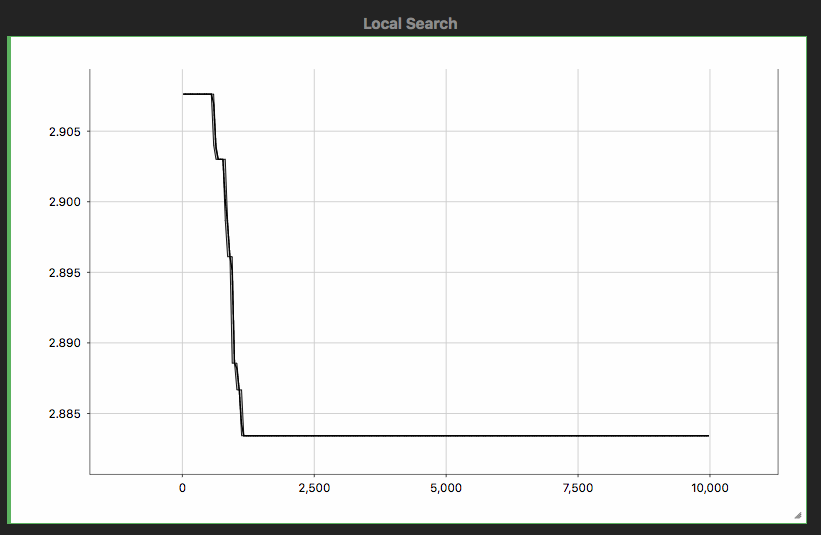
\includegraphics[width=150mm]{Local.png}
    \caption{Búsqueda Local}
    \label{fig:local}
\end{figure}

\section{Algoritmo Genético}

Debido a que la optimización Multi-objetivo se encuentra dominada en la literatura por algoritmos genéticos, resulta relevante usar un algoritmo genético mono-objetivo para hacer una comparación más directa, ya que ambos comparten parámetros como los algoritmos de mutación y crossover además de un épsilon para la evaluación de las soluciones. Como podemos ver en los resultados estas soluciones resultan ser mejores que las obtenidas por búsqueda local y si observamos la muestra de una de las soluciones es evidente ver que la estabilidad del grupo resulta mejor comparada con la que resultaría de un grupo generado de forma aleatoria.

\begin{figure}
    \centering
    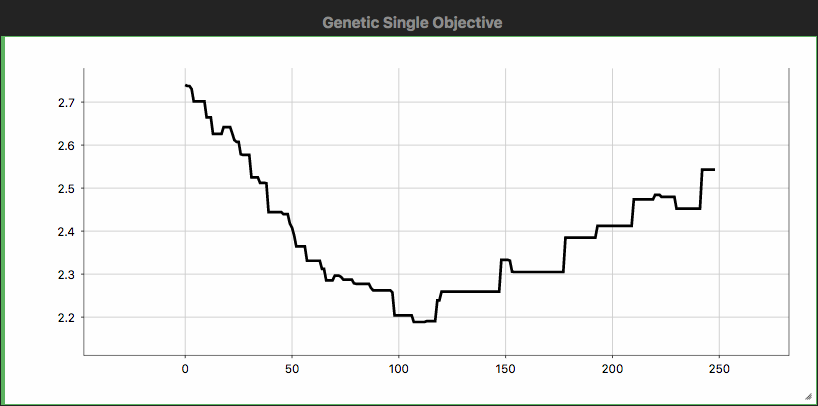
\includegraphics[width=150mm]{Genetic.png}
    \caption{Algoritmo Genético Mono-objetivo}
    \label{fig:genetico}
\end{figure}

\section{Optimización Multi-Objetivo}

Para la optimización multiobjetivo se utilizó el algoritmo NSGA-II qué significa... ya que es uno de los más usados en la literatura de hoy en día, además de que no necesitan parámetros adicionales a los usados para el algoritmo genético de optimización mono-objetivo.

Es posible ver en estos resultados que las soluciones obtenidas por la optimización multiobjetivo resultan ser significativamente mejores, ya que al sumar los valores de las soluciones resultan ser menores a las obtenidas por una optimización mono-objetivo por algoritmos genéticos.

\begin{figure}
    \centering
    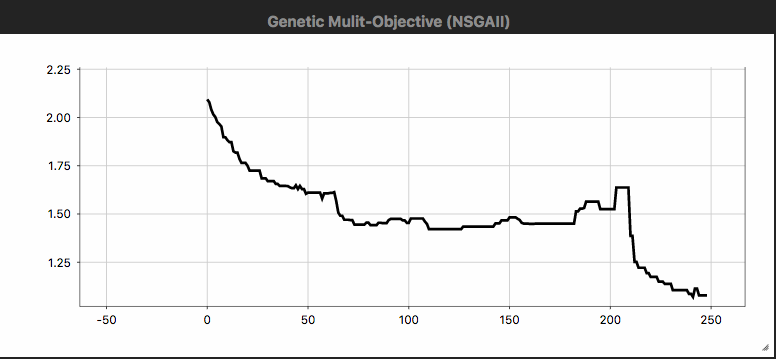
\includegraphics[width=150mm]{Multi-Objective.png}
    \caption{Multi-Objetivo (NSGAII)}
    \label{fig:multiobjetivo}
\end{figure}
